\documentclass[a4,11pt]{article}

\parindent=10pt
\parskip=6pt
%\usepackage[width=15.5cm, left=2.5cm, top=2cm, height= 24.5cm]{geometry}
\usepackage[paper=a4paper, left=2cm, right=2cm, bottom=2.5cm,top=2.5cm]{geometry}

% Paquetes de nacionalización. No olvidar para poder poner tildes!
\usepackage[spanish]{babel}
\usepackage[utf8]{inputenc}

% Paquetes para graficos
\usepackage{subfig}
% \usepackage{graphicx} %% La caratula lo incluye

% Paquetes para matematica
\usepackage{amsmath}
\usepackage{amsfonts}
\usepackage{amssymb}

% Paquetes para pseudo
\usepackage{algorithm}
\usepackage{algorithmic}

% Caratula (Recordar logo_uba.jpg y logo_dc.jpg)
\usepackage{caratula}

% Paquetes para tablas
\usepackage[table]{xcolor}

% Se pueden sacar?
\usepackage{url}
\usepackage{float}
\usepackage{afterpage}
\usepackage{tabularx}

% Color de links
\usepackage{hyperref}
\hypersetup{
    colorlinks,
    citecolor=black,
    filecolor=black,
    linkcolor=black,
    urlcolor=black
}

\begin{document}


\materia{Metodos numericos}
\submateria{Primer Cuatrimestre de 2015}
\titulo{Trabajo Pr\'actico 1}
\subtitulo{“Scheduler”}
\integrante{Ricardo Colombo}{156/08}{ricardogcolombo@gmail.com}
\integrante{Franco Negri}{893/13}{franconegri2004@hotmail.com}
\integrante{Federico Suarez}{610/11}{elgeniofederico@gmail.com}

\maketitle
\pagebreak
  
\tableofcontents

\pagebreak

\section{Introduccion teorica}

\subsection{Preambulo}
El objetivo de este trabajo practico será la implementacion y la experimentacion sobre diversos tipos de schedulers. El proposito de esto será ver cuales son sus ventajas, cuales sus desventajas y cual es más conveniente para determinado set de tareas.
\\
Para ello contaremos con un simulador que actuará como un sistema operativo y que entregará tareas para que cada scheduler corra. Estas tareas serán definidas de antemano, pudiendo simular en ellas un uso intensivo del CPU o una llamada bloqueante del sistema que equivaldrá a que la tarea deba esperar algun recurso del sistema.
\\
Para este trabajo implementaremos un scheduler Round Robin simple, un Round Robin que no permita la migración de procesos entre nucleos, más otros dos schedulers descriptos en el paper de C. L. Liu. Además la cátedra nos provee de un scheduler First Come First Served que utilizaremos para comparar los otros schedulers y sacar conclusiones de los mismos.
\subsection{Metricas a utilizar}

Para medir que tan 'buenos' son los algoritmos utilizados, empelaremos dos metricas distintas: Turnaround y Waiting Time.
\\
Turnaround hará referencia a cuanto tarda un proceso en terminar de ejecutarse desde la primera vez que esta en ready. Esta metrica será buena para medir procesos que utilicen muchos recursos de la CPU ya que esta fuertemente ligado a cuanto quantum esta asignandole el procesador a ese proceso en particular.
\\
La segunda metrica sera Waiting time, y será util para medir tareas que permanezcan mucho tiempo bloqueadas, ya sea por llamadas al sistema, esperen algun input en especial, etc. Es claro que estas tareas no dependen de su tiempo de ejecucion sino de que sean atendidas lo mas rapidamete posibles, O por decirlo de otra manera, se buscará minimizar el tiempo entre que una tarea deja de estar bloqueada y su nueva ejecución.
\\
El lector puede notar que estas dos metricas son bastante contradictorias ya que, para minimizar el turnaround uno tenderia a asignarle la mayor cantidad de recursos posibles a una tarea especifica. Pero esto probocara que las demas tareas no sean atendidas y permanezcan mucho tiempo a la espera. Por otra parte para intentar mejorar el waiting time uno podria elegir un quantum pequeño para cada una de las tareas y que se rote entre ellas de manera constante. Esto sin duda probocará que el procesador este realizando constantes context switches y probocara un peor tiempo en el turnarround.
\\
A manera de introducción, en la siguiente sección se implementarán algunas tareas simples las cuales correremos sobre el scheduler provisto por la catedra para intentar sacar alguas conclusiones preliminares.
\subsection{Experimentacion Preliminar Sobre Scheduler FCFS}

Para esta experimentación primero implementaremos una tarea a la que denominaremos TaskConsola, que simulará una tarea interactiva. La misma contara con $n$ llamadas bloqueantes al sistema de un tiempo aleatorio pasado por parámetro.

La tarea TaskConsola es una función que recibe tres parámetros, el número $n$ de llamadas bloqueantes que debe realizar y las cotas superior e inferior que puede tener el intervalo aleatorio, $bmin$ y $bmax$. Una vez dentro de la función se cicla $n$ veces calculando el intervalo aleatorio en cada iteración y realizando una llamada bloqueante en cada caso con la duración correspondiente.
\\
Luego crearemos un lote de tareas a ejecutar por el simulador, una que utilice de manera intensiva el CPU, y dos TaskConsola. Se realizará una simulación para uno, dos y tres núcleos.
\\
Lo obtenido puede verse en los siguientes gráficos:
\\
\begin{figure}[H]
  \centering
	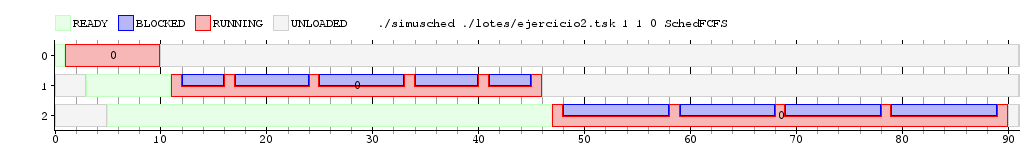
\includegraphics[scale=0.45]{graficos/parte1/testFCFS1.png}
  \caption[Caption for LOF]{}
\end{figure}
\begin{figure}[H]
  \centering
	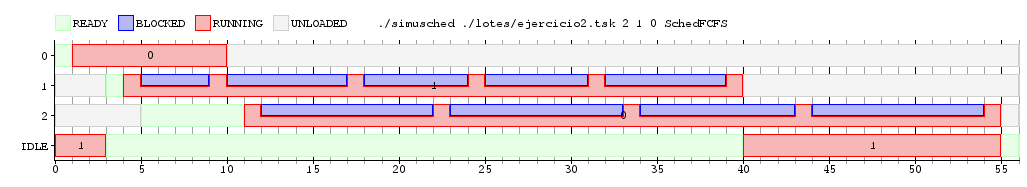
\includegraphics[scale=0.45]{graficos/parte1/testFCFS2.png}
  \caption[Caption for LOF]{}
\end{figure}
\begin{figure}[H]
  \centering
	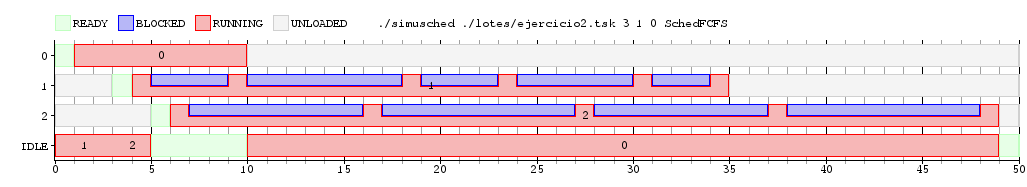
\includegraphics[scale=0.45]{graficos/parte1/testFCFS3.png}
  \caption[Caption for LOF]{}
\end{figure}

En el caso de un núcleo puede verse a simple vista cuál es uno de los problemas fundamentales con este scheduler. Cuando la tarea 1 está bloqueada en espera de algún recurso, el procesador, en vez de cambiar de tarea e intentar adelantar alguna otra, no está siendo utilizado para nada lo que es sin duda una desventaja tanto para el turnaround, ya que otras tareas podrían terminar antes si se ejecutaran, como para el waiting time, ya que se ve claramente que la tarea 2 está teniendo que esperar un gran tiempo sin ser ejecutada.
\\
En los casos de dos y tres núcleos, si bien pueden correrse dos o tres tareas simultáneamente, el 'desperdicio' de procesador por cada núcleo sigue siendo el mismo ya que al hacerse una llamada bloqueante no se desaloja la tarea dándole lugar a otra, sino que el CPU queda ocupado.
\\
Además, cuando se tiene sólo un núcleo, si se diera el caso en que un gran numero de tareas esten esperando para ser ejecutadas, y la primera tarea, por la razón que sea, nunca terminara, entonces todas las demás tareas sufrirían de inanición.
\\
Aún así este tipo de scheduler puede ser útil, ya que es muy fácil de implementar y es posible hacerlo en sistemas donde no se cuentan con interrupciones temporales de las que el kernel pueda hacer uso.
\\
En los siguientes apartados pasaremos a describir e implementar varios schedulers de mayor complejidad que intenten lidiar con los problemas descriptos anteriormente, esto es, schedulers que permitan aprovechar los tiempos muertos en los que la tarea en ejecución debe esperar por algún recurso y que tenga cierto grado de 'justicia' para que ninguna tarea sufra de inanición. Además realizaremos diversas experimentaciones para ver que ventajas y desventajas existen con la utilización de cada uno.


\pagebreak
\section{Desarrollo}

\subsection{Round Robin simple}
El primer scheduler implementado fue el Round Robin. La idea de este scheduler es asignarles a todas las tareas un mismo quantum e ir ejecutándolas de manera circular. En nuestra implementación existe un quantum para cada CPU, lo cual es representado por un arreglo. Los quantum para cada núcleo son parámetros del scheduler. Además, tenemos un contador de ticks para cada núcleo, representado por un arreglo, y una lista de tareas en Ready que se representan con una cola. En cada tick de cada CPU sumo el contador de ticks correspondiente y me fijo si alcanzó el quantum para ese CPU, si así lo hizo entonces desalojo la tarea, la coloco en la cola de Readys, y pongo a correr la siguiente tarea de la cola si es que la hay, y si no, no hago nada y dejo corriendo a la tarea actual. Y por último en los casos que una tarea se bloquea o termina de ejecutar, simplemente llevo a ejecución la siguiente tarea de la cola de Readys si es que la hay.
\\
Para ejemplificar este scheduler, supongamos que tenemos dos tareas, $1$ y $2$, y tan sólo un procesador. La idea de este algoritmo será poner a correr la tarea $1$ durante un tiempo definido por el $quantum$ correspondiente al procesador en el que esté ejecuntándose y pasado ese tiempo, desalojar a esa tarea, y poner a correr a la tarea $2$. Una vez pasado el $quantum$ asignado a la tarea $2$, ésta se desaloja y se pone a correr nuevamente a la tarea $1$. De esta manera nos aseguramos que ninguna tarea sufra de inanición y que todas tengan un progreso más o menos parejo.
\\
Como una prueba preliminar, corrimos el lote diseñado para el algoritmo de First Come First Served para obtener una comparacion razonable entre ellos. Lo que se obtubo para este caso puede verse en el siguiente grafico:
\\
%./simusched tsks/ejercicio2.tsk 1 1 1 SchedRR 5
\begin{figure}[H]
  \centering
	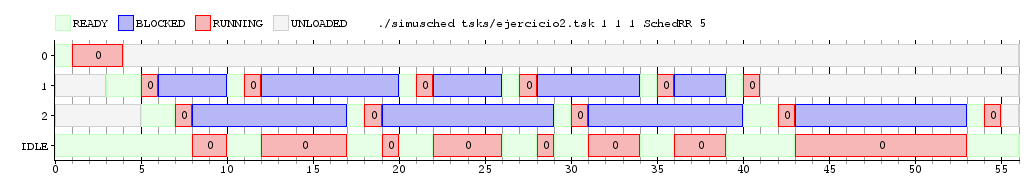
\includegraphics[scale=0.45]{graficos/parte2/rr/1.png}
  \caption[Caption for LOF]{}
\end{figure}
Puede verse que ahora estamos mejorando el turnaround, ya que aprovechamos de mejor manera los tiempos en que una de las tareas esta bloquada. Tambien vemos que este scheduler mejora el waiting time, ya la ejecucion del proceso 3 se hace a la par que la del proceso 2, haciendo que las tareas 1 y 2 esten mucho menos tiempo en ready.
\\
Ahora realizamos otras experimentacines para este scheduler para ver en cuáles casos resulta ser un buen scheduler y en qué casos no.
\\
Para poder visualizar claramente lo que el procesador esta haciendo, en primera instancia, simularemos un solo procesador con un cambio de contexto igual a 1 y un quantum de 5.
\\
Como primer lote corrimos 5 tareas de CPU intensivo y una tarea que tarda mucho en ejecutarse. Para un quantum razonable, puede observarse cómo cada tarea obtiene su quantum (igual a 5) y luego se pasa a la siguiente.
\\
%./simusched tsks/lote1rr.tsk 1 1 1 SchedRR 5
\begin{figure}[H]
  \centering
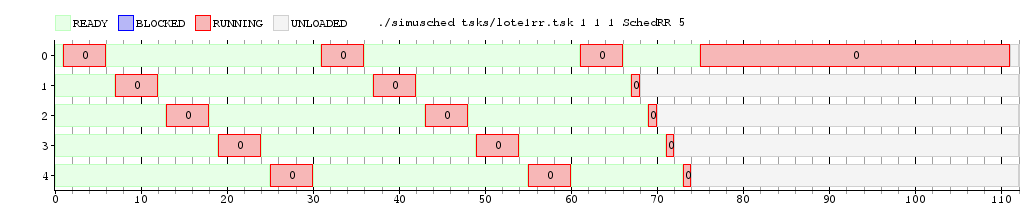
\includegraphics[scale=0.45]{graficos/parte2/rr/2.png}
  \caption[Caption for LOF]{}
\end{figure}
En este test podemos observar que el waiting time es bastante grande para todas las tareas. El turnarroud tambien es bastante amplio para tareas con un tiempo de ejecucion no tan elevado. Sin embargo a pesar de eso puede notarse la principal caracteristica de este algoritmo de scheduling y es que todas las tareas reciben el mismo tiempo de procesamiento y en un orden circular que asegura que ninguna sufra de starvation.
\\
El segundo lote que probamos fue una tarea taskCPU con 4 repeticiones que arranca en el tiempo 3 que aparecen cada 10 ticks de duración 3. Otra tarea taskIO que arranca en el tiempo 6 tarda 4 CPU y 2 de uso IO. Quantum 6.
\\
%./simusched tsks/lote2rr.tsk 1 1 1 SchedRR 5
\begin{figure}[H]
  \centering
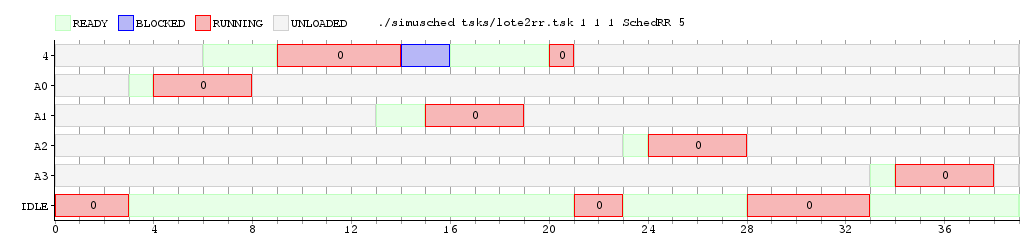
\includegraphics[scale=0.45]{graficos/parte2/rr/3.png}
  \caption[Caption for LOF]{}
\end{figure}
En este experimento podemos ver que este algoritmo puede dar muy buenos resultados tanto en turnaround como en waiting time para un si se utiliza el quantum adecuado. Aun asi cabe notar que este quantum dependerá mucho de que tipo de tareas se esten corriendo y cual sea el tiempo de ejecucion total de cada una de ellas, que puede resultar muy dificultoso de saber a priori. 
\\
Luego de analizar el caso de un solo procesador, decidimos agregar más procesadores para ver qué sucedería y notamos que en este caso se abren varias ramas que vale la pena investigar para entender con más detalle cómo se comporta el algoritmo de round robin, ya que se agregan variables que afectan directamente los tiempos de procesamiento como lo son el costo de cambio de contexto y el costo de cambio de procesador que en el caso de un procesador no se nota ya que el unico que afecta es el cambio de contexto.
\\
Analicemos primero el caso de tener varios procesadores con un costo de cambio de contexto y de procesador ideal, o sea 0 para ambos. Queremos ver cómo se comporta el procesador en este caso y analizar los resultados suponiendo que al haber migración de procesos entre CPUs podemos ver que se aprovecha más el tiempo de procesamiento de los mismos y que en un contexto donde muchas tareas estén corriendo al mismo tiempo será menor el tiempo que un procesador esté corriendo la tarea IDLE, haciendo eficiente el procesamiento de tareas largas simultáneas. Para ello vuelvemos a usar el test de 5 tareas de CPU intensivas con un quantum de 4 para ambos procesadores.
\\
%./simusched tsks/lote1rr.tsk 2 0 0 SchedRR 4 4
\begin{figure}[H]
  \centering
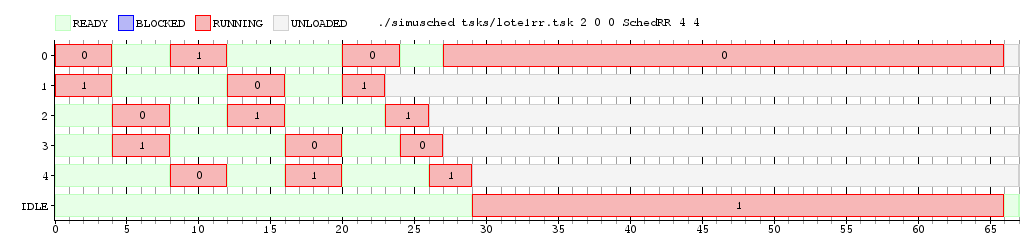
\includegraphics[scale=0.45]{graficos/parte2/rr/4.png}
  \caption[Caption for LOF]{}
\end{figure}
Puede verse que para este caso, el algoritmo de Round Robin se desempeña muy bien, permitiendo que las tareas cortas terminen antes y distribuyendo de manera pareja los procesadores aprovechando su intercambio de procesos resulta optimo para este set.
\\
En el segundo test, analizamos el caso de tener un costo en el cambio de contexto que no sea cero y que el cambio de procesador sea ideal. A simple vista, sin ejecutar un test, podemos imaginar que al no ser nulo el cambio de contexto, el rendimiento se verá afectado por la pérdida de tiempo en los cambios entre tareas, dependiendo del set de tareas y del quantum del procesador. Para el caso de todos procesadores con un quantum grande y un set de tareas chico se podrá ver que el cambio de contexto es despreciable si las tareas se ejecutan todas dentro del quantum de los procesadores. Dicho de otra manera, si todas las tareas tienen un tiempo de ejecución menor al quantum mínimo entonces el tiempo de cambio de contexto será despreciable.
\\
%./simusched tsks/lote1rr.tsk 2 2 0 SchedRR 11 11
\begin{figure}[H]
  \centering
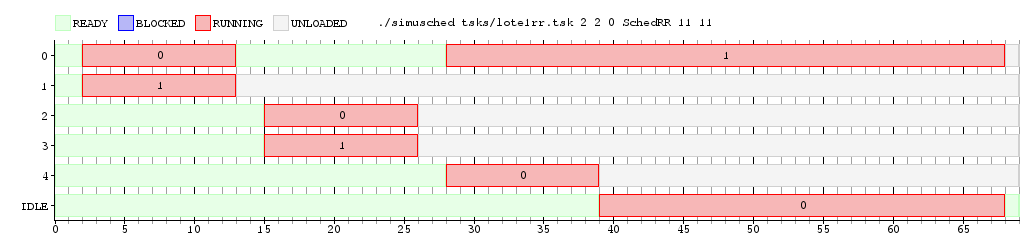
\includegraphics[scale=0.45]{graficos/parte2/rr/5.png}
  \caption[Caption for LOF]{}
\end{figure}
Ahora notemos que en ese caso es muy parecido al cambio de contexto de valor ideal, pero ahora si tenemos un set en el cual una tarea ya supera el quantum minimo entonces se comenzara a notar ese cambio de contexto dentro del factor de procesamiento, peor aun si todas las tareas superan el quantum minimo comenzara a notarse mas.
\\
\begin{figure}[H]
  \centering
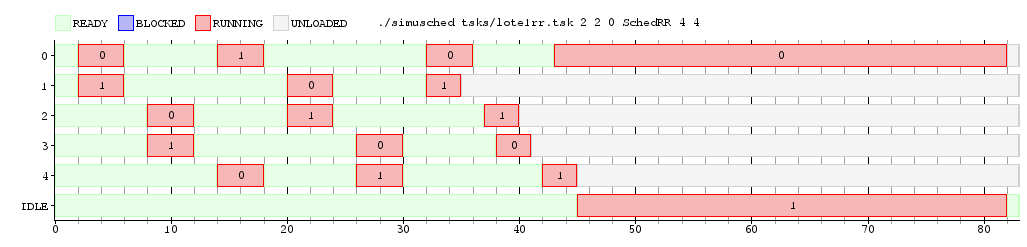
\includegraphics[scale=0.45]{graficos/parte2/rr/6.png}
  \caption[Caption for LOF]{}
\end{figure}
Por ultimo realizamos el mismo tipo de analisis agregandole que el cambio de nucleo de procesamiento no sea nulo y podremos ver que el factor de procesamiento del scheduler sigue aumentando.
%./simusched tsks/lote1rr.tsk 2 2 2 SchedRR 4 4
\begin{figure}[H]
  \centering
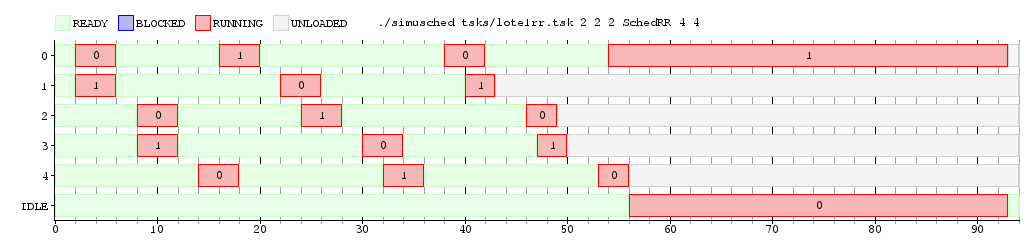
\includegraphics[scale=0.45]{graficos/parte2/rr/7.png}
  \caption[Caption for LOF]{}
\end{figure}
En el siguiente apartado presentaremos una modificacion posible al Round Robin para mitigar este problema que surge cuando la migracion entre procesadores empieza a tener un costo no desprecialbe.
\subsection{Round Robin Sin Migracion Entre CPUs}
La idea detras de este scheduler es basicamente la misma que en el round robin, con el agregado de que cada tarea esta sujeta a un procesador. Esto significa, si la tarea $1$ fue asignada al procesador $1$, solo podrá correr en este procesador. Las tareas se iran asignando para que la carga de las mismas sea siempre sea  pareja entre todos los procesadores en terminos de cantidad de tareas asignadas a cada procesador, no haya uno que se encargue de todas las tareas y otro al que no se le asigne ninguna.De esta manera podremos aprovechar cada cola de procesamiento y analizar segun que set de tareas el algoritmo es bueno con respecto a los demas.
\\
La principal ventaja de esta implementacion es que habra un mejor uso de la caché, en caso de poseer cache en varios niveles teniendo cache por procesador y una compartida, ya que si la tarea $1$ corria en el procesador $1$ y fue desalojada, al volver a ejecutarse, si es en el procesador $1$ puede darse el caso en que sus datos continunen cacheados, mientras que si se le asigna otro CPU tendrá que cargar todos los datos nuevamente, por lo que al no haber un cambio de tareas entre procesadores se eliminara el tiempo de cambio de proceso entre nucleos  pero no sera eliminado el tiempo de cambio de contexto.
\\
Ahora si volvemos a ejecutar el ultimo test del apartado anterior, con la misma cantidad de procesadores y mismos parametros, esperamos obtener reslutados mejores:
\\
\begin{figure}[H]
  \centering
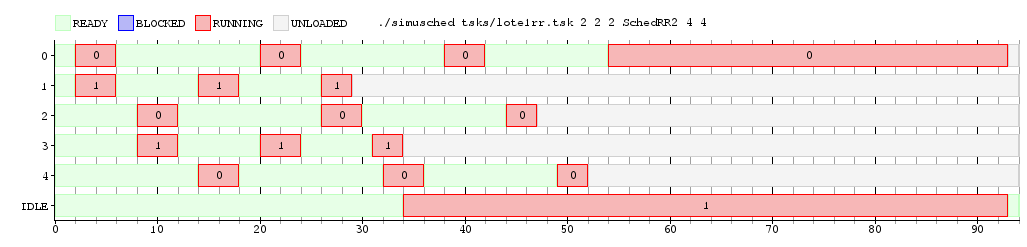
\includegraphics[scale=0.45]{graficos/parte2/rr2/1.png}
  \caption[Caption for LOF]{}
\end{figure}
Efectivamente ahora podemos observar que para el mismo set de tareas obtuvimos una mejora de 5 ticks en el proceso 4 y alrededor de 10 ticks para el proceso 2. Como desventaja de este algoritmo puede verse que en este caso uno de los procesadores estará ocioso mucho más tiempo que en la implementación del Round Robin simple.
\subsection{Comparando implementaciones de Round Robin}
Para la comparación entre el Round Robin con migración entre CPUs y sin migración con CPUs, buscamos primero encontrar set de tareas en los cuales sea mejor el Round Robin con el cambio de procesos entre CPUs y otro caso donde sea mejor el algoritmo sin el intercambio de procesos entre CPUs.
\\
Para el primer caso encontramos un conjunto donde tenemos 3 tareas de las cuales dos son de un procesamiento muy extenso y la tercera es de un procesamiento muy corto las cuales las programamos para que al inicio ingrese una de las tareas con mucho tiempo de ejecución seguida por la que tiene un corto tiempo de ejecución y para terminar la faltante mientras se procesan las dos primeras, esto era fue algo que mencionamos anteriormente como ventaja.
\\
\begin{figure}[H]
  \centering
%./simusched tsks/rrVsrr2.tsk 2 2 2 SchedRR 4 4
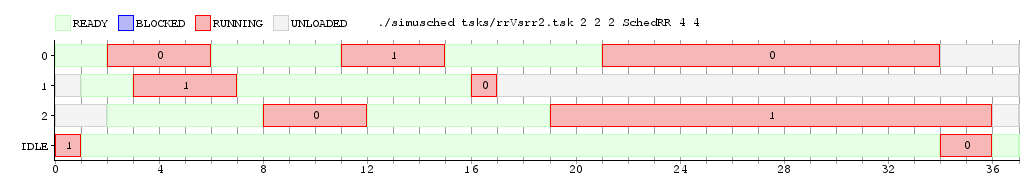
\includegraphics[scale=0.45]{graficos/rrVsrr2/1.png}
  \caption[Caption for LOF]{Scheduler RR simple}
\end{figure}
\begin{figure}[H]
  \centering
%./simusched tsks/rrVsrr2.tsk 2 2 2 SchedRR2 4 4
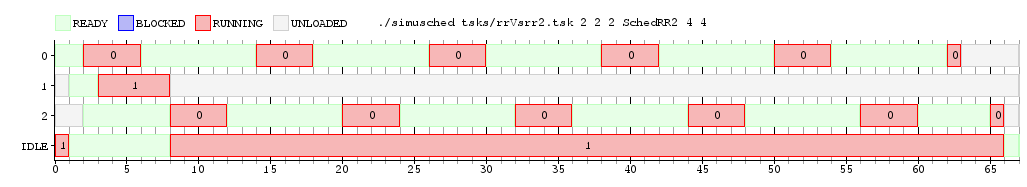
\includegraphics[scale=0.45]{graficos/rrVsrr2/2.png}
  \caption[Caption for LOF]{Scheduler RR sin desalojo}
\end{figure}
Como notamos en la comparativa podemos ver que el RR sigue siendo más eficiente que el RR2 para la ejecución de tareas largas, ya que en este caso el RR2 mientras que el procesador 0 ejecuta las tareas largas el otro procesador queda en estado IDLE perdiendo todo ese tiempo en ejecutar la otra tarea.
\\
\\
\begin{figure}[H]
  \centering
%../simusched tsks/rrVsrr2.2.tsk 2 2 2 SchedRR 4 4
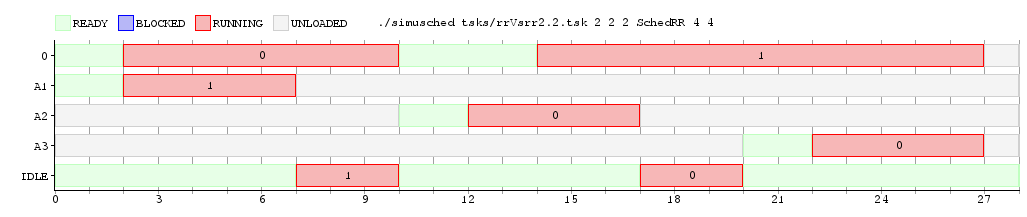
\includegraphics[scale=0.45]{graficos/rrVsrr2/3.png}
  \caption[Caption for LOF]{Scheduler RR simple}
\end{figure}
\begin{figure}[H]
  \centering
%./simusched tsks/rrVsrr2.2.tsk 2 2 2 SchedRR2 4 4 
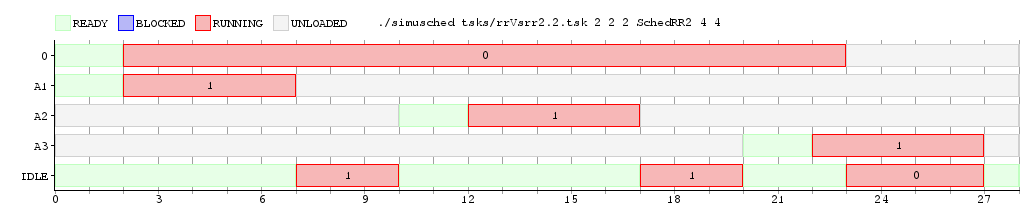
\includegraphics[scale=0.45]{graficos/rrVsrr2/4.png}
  \caption[Caption for LOF]{Scheduler RR sin desalojo}
\end{figure}
Como podemos ver en los gráficos el Round Robin sin migración de CPUs tiene un menor waiting time y un mejor turnaround para el proceso 0. Mientras que las demás tareas continuan teniendo los mismos tiempos de ejecución. Por lo que podríamos concluir que para este caso es mejor el Round Robin sin migración entre CPUs.
\\
\section{Paper Scheduling Algorithms for Multiprogramming in a Hard Real Time Enviroment by C. L. Liu}
\subsection{Problema}

En los sistemas de tiempo real, los procesos que se corren son llamados en respuesta a ciertos eventos que suceden periódicamente y deben finalizarse antes de un determinado tiempo crítico, con lo cual, el que estos tiempos puedan satifascerse de manera eficiente depende en una gran medida del algoritmo de scheduling que se utilice, es decir, que éste pueda organizar los procesos de manera tal que todos cumplan sus tiempos.

En este paper se enseñan tres algoritmos para este tipo de sistemas, pero nosotros sólo nos enfocaremos en la implementación y el estudio de dos de ellos.

A continuación desarrollaremos dos ideas de scheduling que se aplican a un entorno en donde hay una cantidad $m$ de tareas que aparecen periódicamente, algo característico en los sistemas de tiempo real. Cada una de estas tareas tiene un período fijo que no varía, es decir, una frecuencia determinada que no cambia, y asimismo tampoco varía el uso de CPU con el correr de las ejecuciones de una misma tarea. Se busca poder organizar las tareas de tal manera que toda respuesta a la llamada de una tarea finalice antes de que llegue la próxima llamada a dicha tarea.

Los siguientes schedulers se basan en prioridades, y como todo scheduler basado en prioridades, cuentan con desalojo, para quitar una tarea que está corriendo cuando una de mayor prioridad ingresa al sistema. Se diferencian entre sí por el criterio para asignar dichas prioridades y el momento en el que éstas se asignan.

\subsection{Scheduler Fixed Para Real Time}
Antes de comenzar la explicación de este algoritmo de scheduling, definamos algunos conceptos importantes. El 'deadline' del llamado a una tarea está dado por el momento en el que llega el siguiente llamado a la misma tarea. Decimos que hay un 'overflow' cuando en un determinado tiempo se realiza un llamado a una tarea cuyo llamado anterior aún no terminó, o sea, cuando una tarea no llega a finalizar antes de que su 'deadline' llegue. Dado un set de tareas, decimos que un algoritmo de scheduling es 'factible' si planifica las tareas de tal manera que no ocurra ningún 'overflow'. Definimos 'tiempo de respuesta' del llamado a una tarea como el tiempo desde que ese llamado ocurre hasta que la tarea finaliza. Un 'instante crítico' de una tarea se define como el instante en el que el llamado a esa tarea tendrá el 'tiempo de respuesta' más largo.

Este scheduler se basa en prioridades fijas, es decir, antes de comenzar la ejecución de un set de tareas, se establecen las prioridades de las mismas. Una vez establecidas las prioridades, comienza la ejecución de las tareas y las prioridades ya no pueden cambiarse y deben respetarse a rajatabla. Las prioridades se asignan en base a la frecuencia de cada tarea periódica, es decir, una mayor frecuencia significa una mayor prioridad, con lo cual aquellas tareas que lleguen más seguido al sistema serán las que mayor prioridad de ejecución tengan. Es importante notar que para que este tipo de scheduler estático sea factible, todas las tareas deben satisfacer sus deadlines en sus instantes críticos.
\\

Para ver a este scheduler en acción y analizar su comportamiento, diseñamos dos sets de tareas para los cuales el scheduling estático sea un algoritmo factible. El primer set se trata de dos familias de tareas periódicas y el segundo de tres familias. A continuación se muestra lo que obtuvimos.

\begin{figure}[H]
  \centering
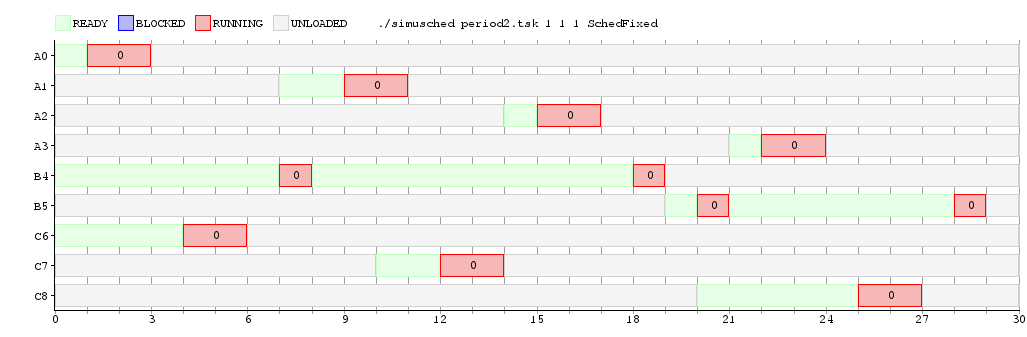
\includegraphics[scale=0.45]{fixed/period2.png}
  \caption[test 1]{}
\end{figure}

Para el primer set se hicieron pocas tareas para ver cómo se comportaba el algoritmo con dos familias, se puede notar que el intercambio de procesador por tarea cumple con los tiempos, es decir, todas las tareas terminan antes de que la siguiente tarea de su misma familia llegue al sistema.

\begin{figure}[H]
  \centering
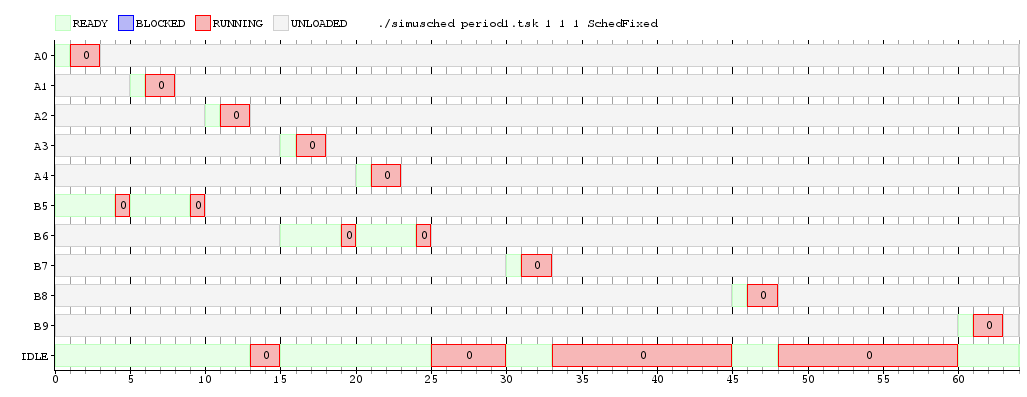
\includegraphics[scale=0.45]{fixed/period1.png}
  \caption[test 2]{}
\end{figure}

En este segundo set de tareas se puede observar que la primer tarea de la familia B, al llegar una de mayor prioridad, es desalojada y vuelve a estar nuevamente en estado ready, pasando a estar en ejecución la tarea recién llegada. Cuando las tareas de mayor prioridad terminan, la tarea de la familia B puede finalizar su ejecución antes de que llegue la próxima tarea de su familia. Cuando deja de haber tareas de la familia A y/o B en ready, entonces es ahí cuando se ejecutan las tareas de la familia C.

Notamos con este algoritmo que preparar las familias sin que ocurra un overflow es difícil en el caso que se quiera ver el intercambio de tareas por prioridad y a su vez se vuelve acotada la cantidad de set de tareas a ejecutar con esta restricción.

\\

\subsection{Problemas del Scheduler Fixed y sección 7}
El factor de utilización del procesador es la fracción de tiempo del mismo dedicada a la ejecucción del set de tareas. Si la fracción de tiempo de procesador dedicado a la ejecución de una tarea $i$ es $C_i$/$T_i$, entonces, para un set de $m$ tareas, el factor de utilización es:
 U = $\sum_{i=1}^{m} (C_{i}/T_{i})$
Este factor de utilización se encuentra acotado superiormente por el requerimiento de que todas las tareas satisfagan sus deadlines en sus instantes críticos. Dada una asignación de prioridades, decimos que un set de tareas 'aprovecha completamente' el procesador si esa asignación de prioridades es factible para el set y cualquier aumento en el tiempo de ejecución de alguna de las tareas del set la vuelve no factible. Para un algoritmo de scheduling dado, la menor cota superior del factor de utilización es el mínimo de los factores de utilización entre todos los set de tareas que 'aprovechan completamente' el procesador. Para todos aquellos set de tareas cuyo factor de utilización del procesador sea menor a esta cota, existe una asignación de prioridades estática que es factible.


\subsection{Scheduler Dynamic Para Real Time}
Este es un scheduler que se basa en prioridades dinámicas, es decir, las prioridades se asignan en el momento siguiendo del criterio elegido. En nuestro algoritmo de scheduling para asignar las prioridades a cada momento se basa en cuál es la tarea con el deadline más cercano, es decir, se les asignará una mayor prioridad a las tareas cuyo deadline sea el más cercano al momento actual. Esto quiere decir que siempre tendrá prioridad de ejecución la tarea más próxima a recibir su siguiente llamado a la misma.Es importante notar que este algoritmo de scheduling maximiza el factor de utilización del procesador, es decir, aproximandolo al 100\%

Para este algoritmo lo que hicimos en la parte de test fue revisar los mismos set de tareas que en el caso del fixed para ver primero cómo se comporta en comparación con el otro algoritmo.


\begin{figure}[H]
  \centering
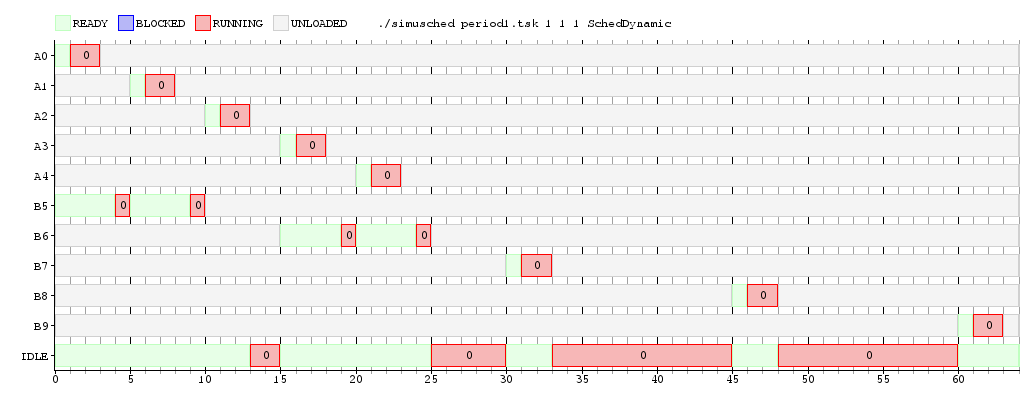
\includegraphics[scale=0.45]{dynamic/period1D.png}
  \caption[Algoritmo Fixed]{}
\end{figure}

\begin{figure}[H]
  \centering
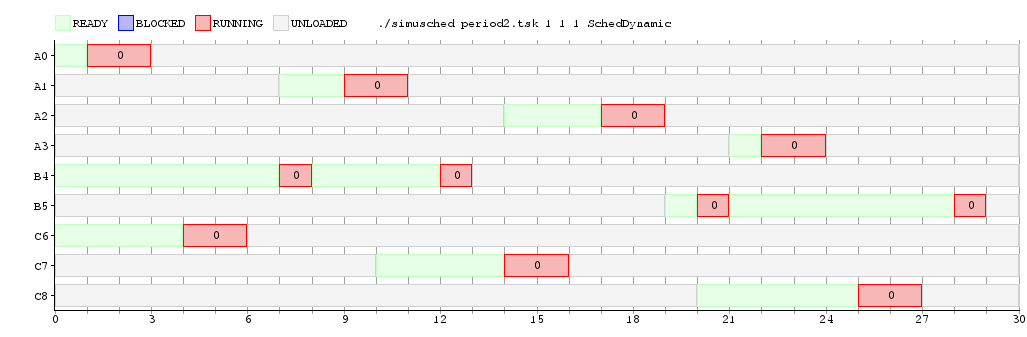
\includegraphics[scale=0.45]{dynamic/period2D.png}
  \caption[Algoritmo Dinamico]{}
\end{figure}

Se puede ver que el algoritmo dinámico se comporta de la misma manera que el fixed para este set. Siendo que no hay overflow era esperable este comportamiento.

Dado el teorema 5 del paper, sabemos que la menor cota superior del factor de utilización del procesador de un algoritmo de scheduling estático es U $=$ $m(2^{1/m}-1)$, siendo ésta aproximable por el ln 2 para un set grande de tareas. Con lo cual lo que se busca es mejorar esta situación, ya que todavía deben tenerse en cuenta los costos prácticos de cambio entre tareas. El algoritmo de scheduling dinámico, que será la solución al problema previamente mencionado, se introduce recién en la sección 7 del paper ya que justo antes se termina de obtener analíticamente la menor cota superior del factor de utilización del procesador de un algoritmo de scheduling y el problema que éste acarrea para sets de tareas muy grandes.


\subsection{Experimentación Comparación Fixed vs Dynamic}

Para terminar con el análisis de los algoritmos decidimos generar un set de tareas que en el fixed no funcionase y ver cómo se comporta el algoritmo dinámico con este mismo set.
Para encontrar un set apropiado para esto se buscó uno que tenga un overflow entre las tareas en el fixed para luego ver cómo el dinámico puede mejorar el manejo del set.

\begin{figure}[H]
  \centering
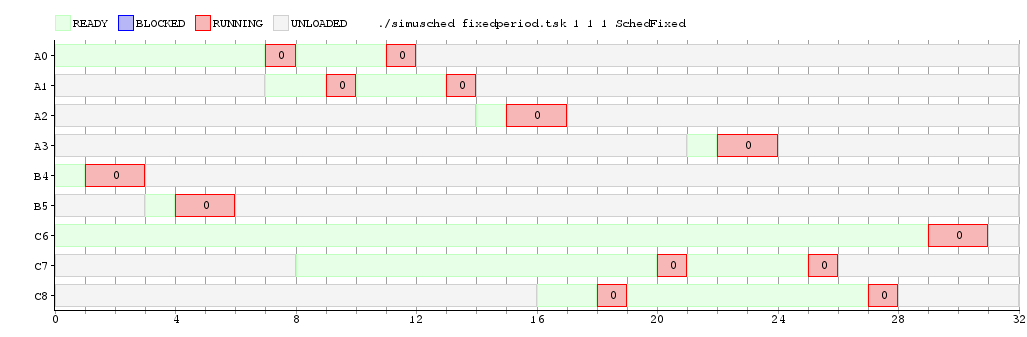
\includegraphics[scale=0.45]{fixedvsdynamic/fD.png}
  \caption[Algoritmo Fixed]{}
\end{figure}

En el caso del Fixed se nota a primera vista que para la familia A hay overflow entre las dos primeras tareas, haciendo que para este set no sea factible el algoritmo estático.

\begin{figure}[H]
  \centering
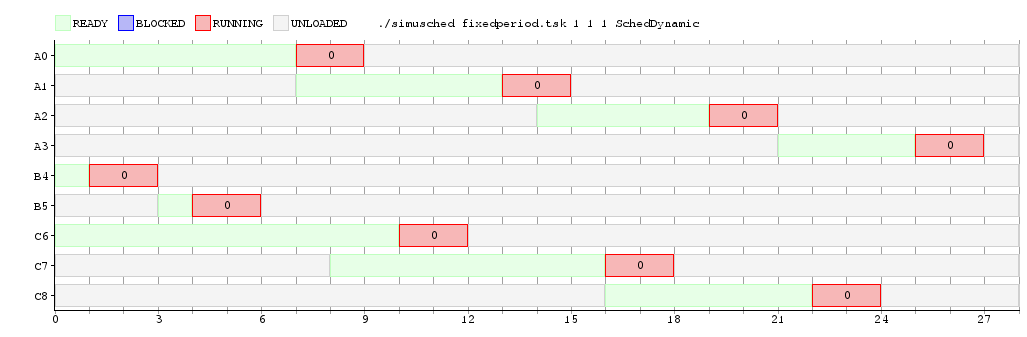
\includegraphics[scale=0.45]{fixedvsdynamic/fD2.png}
  \caption[Algoritmo Dinamico]{}
\end{figure}

Acá se puede ver cómo el mismo set de tareas que para el algoritmo Fixed no es factible, para el algoritmo dinámico sí lo es. Lo manejó sin problemas, pudiendo ejecutar las dos familias ajustando las prioridades de tal forma que no haya overflow.

Como mencionamos anteriormente, el algoritmo Fixed acota con sus limitaciones el set de tareas a ejecutar, haciéndolo bueno en pocas ocasiones.

\subsection{Teorema 7}
El Teorema 7 dice que dado un set de $m$ tareas, el algoritmo de scheduling dinámico es factible si y solo si ($C_1$/$T_1$) + ($C_2$/$T_2$) + ... + ($C_m$/$T_m$) $\le$ 1. Lo que esto nos dice es que el factor de utilización del procesador de este algoritmo de scheduling no debe pasar de 1, o sea, si se tiene un set de tareas en el cual la demanda de cómputo total es mayor al tiempo disponible del procesador entonces el algoritmo de scheduling dinámico no es factible para ese set de tareas ya que al no haber suficiente tiempo de procesamiento disponible, el overflow es inevitable.



\pagebreak
\section{Conclusiones}

Como concluciones para este trabajo practico podemos decir que el scheduler es algo muy dependiente de que estemos intentando lograr con el. Vimos que para siertos casos un round robin puede darnos un buen waiting time y un buen turaround, siempre y cuando el quantum sea adecuado y la migracion de procesos entre CPUs sea despreciable. En caso de no serlo, el Round Robin puede obtener mejores reslutados siempre y cuando no se presenten tareas patologicas que produzcan que un procesador este sobrecargado y otro no tenga tareas para ejecutar.
\\
Por otra parte si lo que se busca es un scheduler de tiempo real que cumpla con deadlines estrictas, puede optarse por alguno de los dos algoritmos descriptos en la segunda parte del trabajo practico ya que nos asegurarán que estas dedlines se cumplan.


\pagebreak
\section{Apendice}


\subsection{Lotes De Tareas }

Dentro de la carpeta SRC se encuentran algunos de los lotes de tareas que usamos para expermentacion.

Ejercicio2.tsk - es el lote utilizado para el ejercicio 2 del trabajo, utilizado en la seccion de desarrollo del round robin.

lote1rr.tsk - es el lote utilizado para la seccion de round robin en el desarrollo y tambien para el round robin sin migracion entre procesadores.

rrvsrr2.tsk y rrvsrr2.2.tsk son los lotes utilizados par comparar los algoritmos de round robin y mostrados en la seccion de comparacion entre los algoritmos.

period1.tsk y period2.tsk son los utilizados en el desarrollo de algoritmos fixed y dynamic.

fixedperiod.tsk es el lote utilizado en la comparacion de algoritmos dynamic y fixed.

taskbatchtest.tsk es el lote utilizado en el ejercicio 7




\end{document}
